
\section{Performance Evaluation}

% Figure reference
\begin{figure}[t]
    \centering
    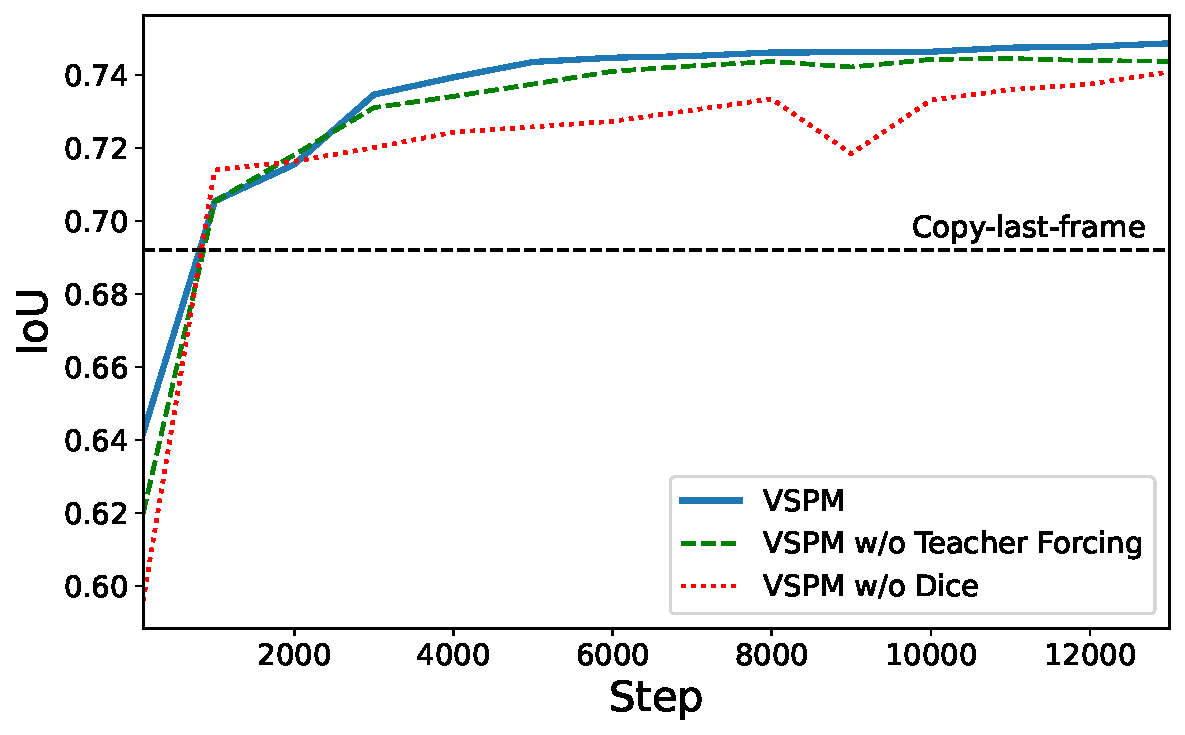
\includegraphics[width=0.95\linewidth]{pics/step-iou.pdf}
    \caption{
        \textbf{Ablation study on prediction IoU across horizons.} 
        Our full vehicle-specific prediction model~(VSPM) achieves consistently higher IoU compared to two ablated variants and a trivial copy-last-frame baseline. The x-axis represents the prediction horizon, and the y-axis represents the IoU score.
    }
    \label{fig:step_iou}
\end{figure}


\begin{figure*}[ht]
    \centering
    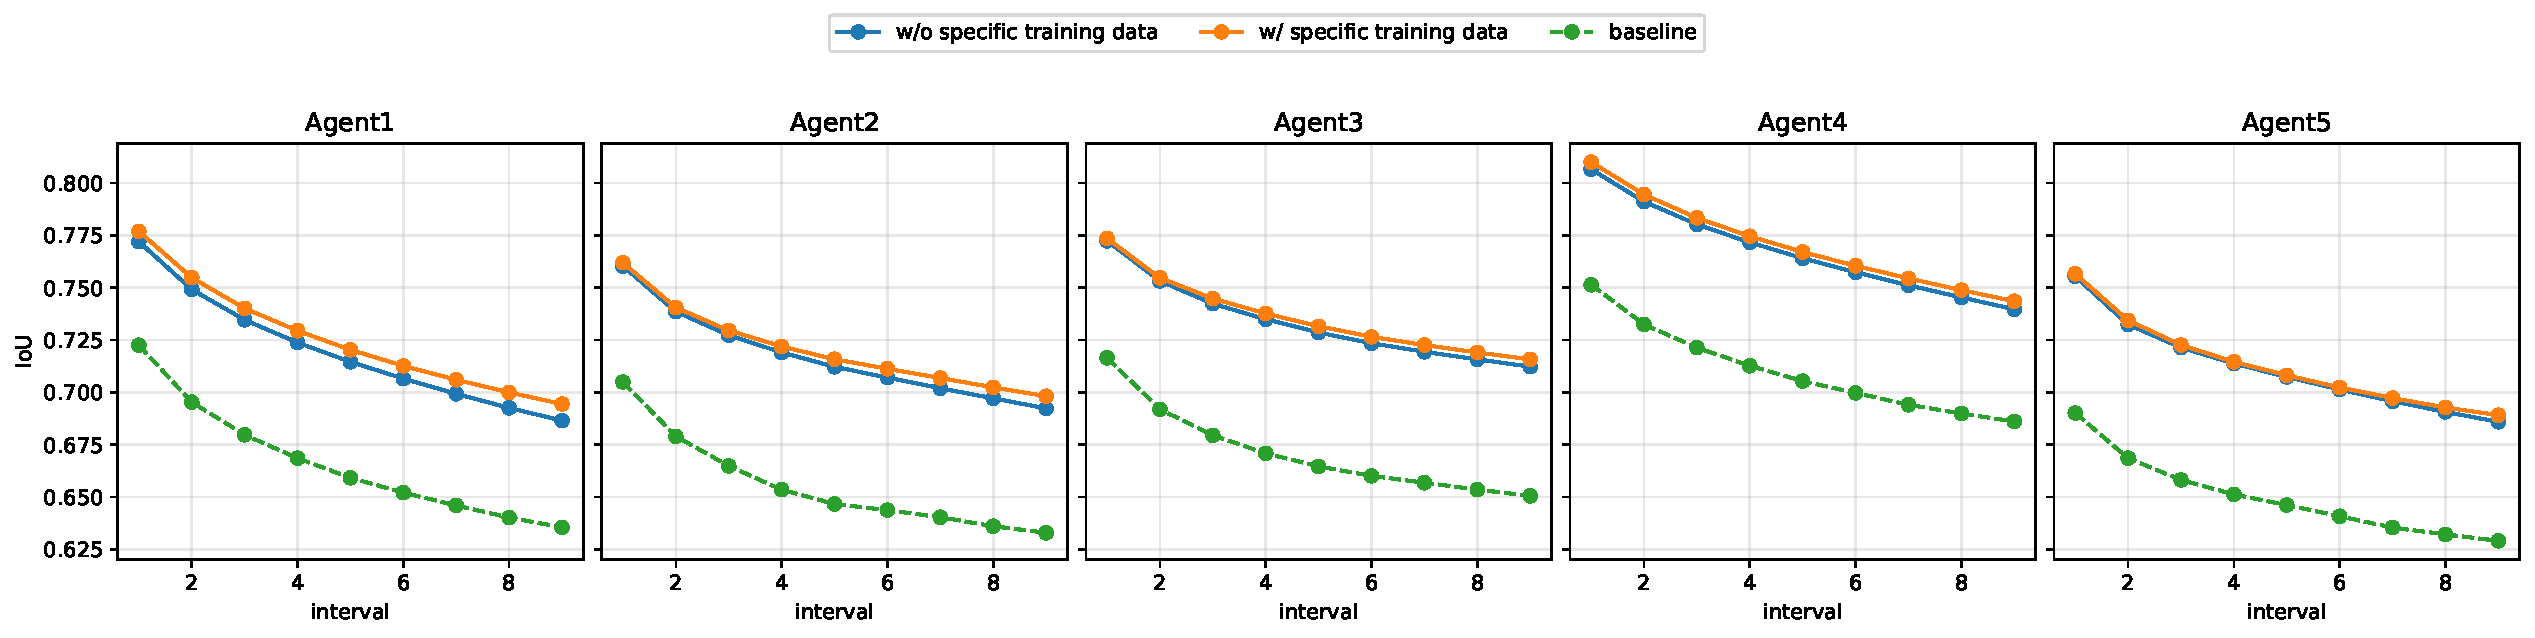
\includegraphics[width=0.95\linewidth]{pics/iou_vs_interval_5agents.pdf}
    \caption{
        \textbf{Comparison of prediction accuracy between generic and personalized models.} 
        IoU is reported under different latency intervals (measured in frames, with each frame representing 0.2 seconds) on the V2X-Sim dataset. Our personalization model consistently outperforms the generic model and the trivial copy-last-frame baseline. 
    }
    \label{fig:iou_interval}
\end{figure*}

\subsection{Experimental setup and evaluation metrics}
We conduct extensive experiments on both the V2X-Sim~\cite{li2022v2x} dataset and the real-world DAIR-V2X-C cooperative perception data to validate the effectiveness of the proposed dual-latency prediction compensation mechanism. Following prior works in cooperative perception, the V2X-Sim training and evaluation are performed on synchronized multi-vehicle data with simulated communication latency and computational latency. Our implementation is built upon the open-source V2VNet~\cite{wang2020v2vnet} and DiscoNet~\cite{li2021learning} framework, where we additionally integrate a lightweight prediction module at the transmitter side to compensate for both communication and computation latencies. For DAIR-V2X-C, we report official point-cloud detection baselines and additionally construct annotation-derived BEV occupancy sequences to evaluate the proposed VSPM and MST modules under real cooperative driving scenes.

For evaluation, we employ three categories of metrics. (1) To assess the accuracy of the vehicle-specific prediction models, we measure the Intersection-over-Union (IoU) between the predicted binary BEV occupancy grids and the ground-truth occupancy maps across different prediction horizons. We also report the IoU gain over the copy-last-frame baseline and the Dynamic IoU on changed BEV regions. (2) To quantify the system-level overhead, we record the reduction in both communication load and computational demand after introducing the proposed transmission scheme. (3) Finally, for the downstream perception fusion performance, we report Average Precision (AP) at IoU thresholds of 0.5 and 0.7, following standard practice in object detection benchmarks.
 



\subsection{Results analysis}
\subsubsection{\textbf{Vehicle-Specific Prediction Model}}
We first evaluate the effectiveness of the proposed prediction module in isolation, without involving any cooperative perception. Specifically, we compare the IoU between predicted and ground-truth occupancy maps under different prediction horizons, as shown in Fig.~\ref{fig:step_iou} and Fig.~\ref{fig:iou_interval}. In addition to conducting a detailed ablation study to quantify the impact of key design choices in our Visual Specific Prediction Module (VSPM), we compare the performance of our VSPM under two different configurations: one as a general model and the other as a specific model, which validates the importance of vehicle-specific in our framework.


\paragraph{Ablation Study}


Our full VSPM integrates scheduled teacher forcing, dynamic per-pixel weighting, and Dice regularization to improve prediction stability in both static and dynamic regions. It represents the main configuration of our model.

\textbf{VSPM w/o Teacher Forcing:}
To study the effect of teacher forcing, we disable scheduled sampling and instead always feed the model's own predictions as decoder inputs during training. This exposes the model to compounding prediction errors during rollout, providing a stress test of exposure bias.

\textbf{VSPM w/o Dice:}  
To examine the effect of addressing class imbalance, we remove the Dice loss while keeping all other components unchanged. Since occupancy prediction often suffers from the sparsity of dynamic objects, this ablation tests the necessity of Dice regularization for improving performance in foreground regions.

\textbf{Copy-last-frame Baseline:}  
We additionally include a trivial baseline that directly copies the previous observed occupancy map as the prediction for future horizons, without any learned dynamics modeling.

Figure~\ref{fig:step_iou} shows the IoU trajectories over prediction horizons. Our full VSPM consistently outperforms both ablations and the trivial baseline across all horizons. Notably, removing teacher forcing leads to a sharp IoU degradation in long-term predictions, while removing Dice yields a moderate performance drop in both near-term and far-horizon forecasts. These results validate the necessity of both components for accurate and stable occupancy prediction.



\paragraph{Effectiveness of VSPM}

Beyond the internal ablations, we further evaluate the overall impact of personalization by comparing three different prediction strategies:  
(1) a \textbf{generic model} trained solely on data from other vehicles without using any vehicle-specific information,  
(2) a \textbf{personalization model} trained on both generic multi-vehicle data and the receiver vehicle's historical data, and  
(3) a \textbf{copy-last-frame baseline} that simply reuses the most recent observation without any learned prediction.


 
As shown in Fig.~\ref{fig:iou_interval}, the personalization model achieves consistently higher IoU across all prediction horizons compared to the generic model and the copy-last-frame baseline. We highlight the following key findings:
\begin{itemize}[leftmargin=*,itemsep=0pt,parsep=0.2em,topsep=0.2em,partopsep=0.0em]
    \item Effectiveness of Personalization: Leveraging vehicle-specific historical data significantly improves prediction accuracy. At a $9$-frame latency, the personalization model consistently achieves higher IoU than the generic model across all scenarios.
    \item Limitations of Generic Models: Without access to the receiver vehicle's historical dynamics, the generic model struggles to adapt to diverse driving behaviors, leading to reduced performance as latency increases.
    \item Baseline Weakness: The copy-last-frame baseline suffers the most severe degradation, particularly for large latency, validating the necessity of learned temporal modeling.
\end{itemize}

These results confirm that VSPM offers a clear advantage over generic models under communication and computation latency constraints.


\begin{table*}[t]
\centering
\caption{Comparison of mAP@0.5 and mAP@0.7 under different \emph{communication and computation latency} settings on the V2X\textendash Sim dataset. Oracle and No Collaboration are reported only at the AVG columns (others are unavailable, shown as ``--''). Our method outperforms V2VNet across all latency conditions and surpasses the Oracle under zero latency.}
\begin{tabular}{c c *{14}{c}}
\toprule
\multirow{2}{*}{\textbf{Method}} & &
\multicolumn{7}{c}{\textbf{AP@0.5}} &
\multicolumn{7}{c}{\textbf{AP@0.7}} \\
\cmidrule(lr){3-9}\cmidrule(lr){10-16}
& \multicolumn{1}{c}{\diagbox{\small{Comp.}}{\small{Comm.}}} &
\textbf{AVG} & \textbf{0} & \textbf{1} & \textbf{2} & \textbf{3} & \textbf{4} & \textbf{5} &
\textbf{AVG} & \textbf{0} & \textbf{1} & \textbf{2} & \textbf{3} & \textbf{4} & \textbf{5} \\
\midrule
\textbf{Oracle} & -- &
\textit{64.91} & -- & -- & -- & -- & -- & -- &
\textit{57.26} & -- & -- & -- & -- & -- & -- \\
\textbf{No Collaboration} & -- &
49.90 & -- & -- & -- & -- & -- & -- &
44.21 & -- & -- & -- & -- & -- & -- \\
\midrule
\multirow{3}{*}{\textbf{V2VNet}} & 0 &
57.43 & 64.91 & 60.01 & 55.69 & 54.44 & 53.79 & 53.21 &
47.61 & 57.26 & 47.03 & 45.46 & 45.24 & 44.78 & 44.51 \\
& 2 &
54.63 & 55.45 & 54.91 & 54.73 & 54.55 & 54.23 & 53.89 &
45.20 & 45.29 & 45.40 & 45.35 & 45.27 & 45.05 & 44.82 \\
& 4 &
53.52 & 53.33 & 53.55 & 53.69 & 53.61 & 53.53 & 53.39 &
44.45 & 44.35 & 44.65 & 44.57 & 44.47 & 44.39 & 44.28 \\
\midrule
\multirow{3}{*}{\textbf{Ours}} & 0 &
64.41 & 67.45 & 65.16 & 64.06 & 63.56 & 63.19 & 63.04 &
56.41 & 58.64 & 57.12 & 56.25 & 55.68 & 55.43 & 55.34 \\
& 2 &
57.01 & 57.54 & 57.22 & 56.97 & 56.91 & 56.78 & 56.63 &
50.45 & 51.02 & 50.64 & 50.42 & 50.36 & 50.22 & 50.03 \\
& 4 &
56.07 & 56.40 & 56.21 & 56.15 & 55.96 & 55.90 & 55.80 &
49.45 & 49.87 & 49.65 & 49.46 & 49.39 & 49.25 & 49.09 \\
\bottomrule
\end{tabular}
\label{tab:map-upper-lower-v2v}
\end{table*}

\begin{figure*}[t]
    \centering
    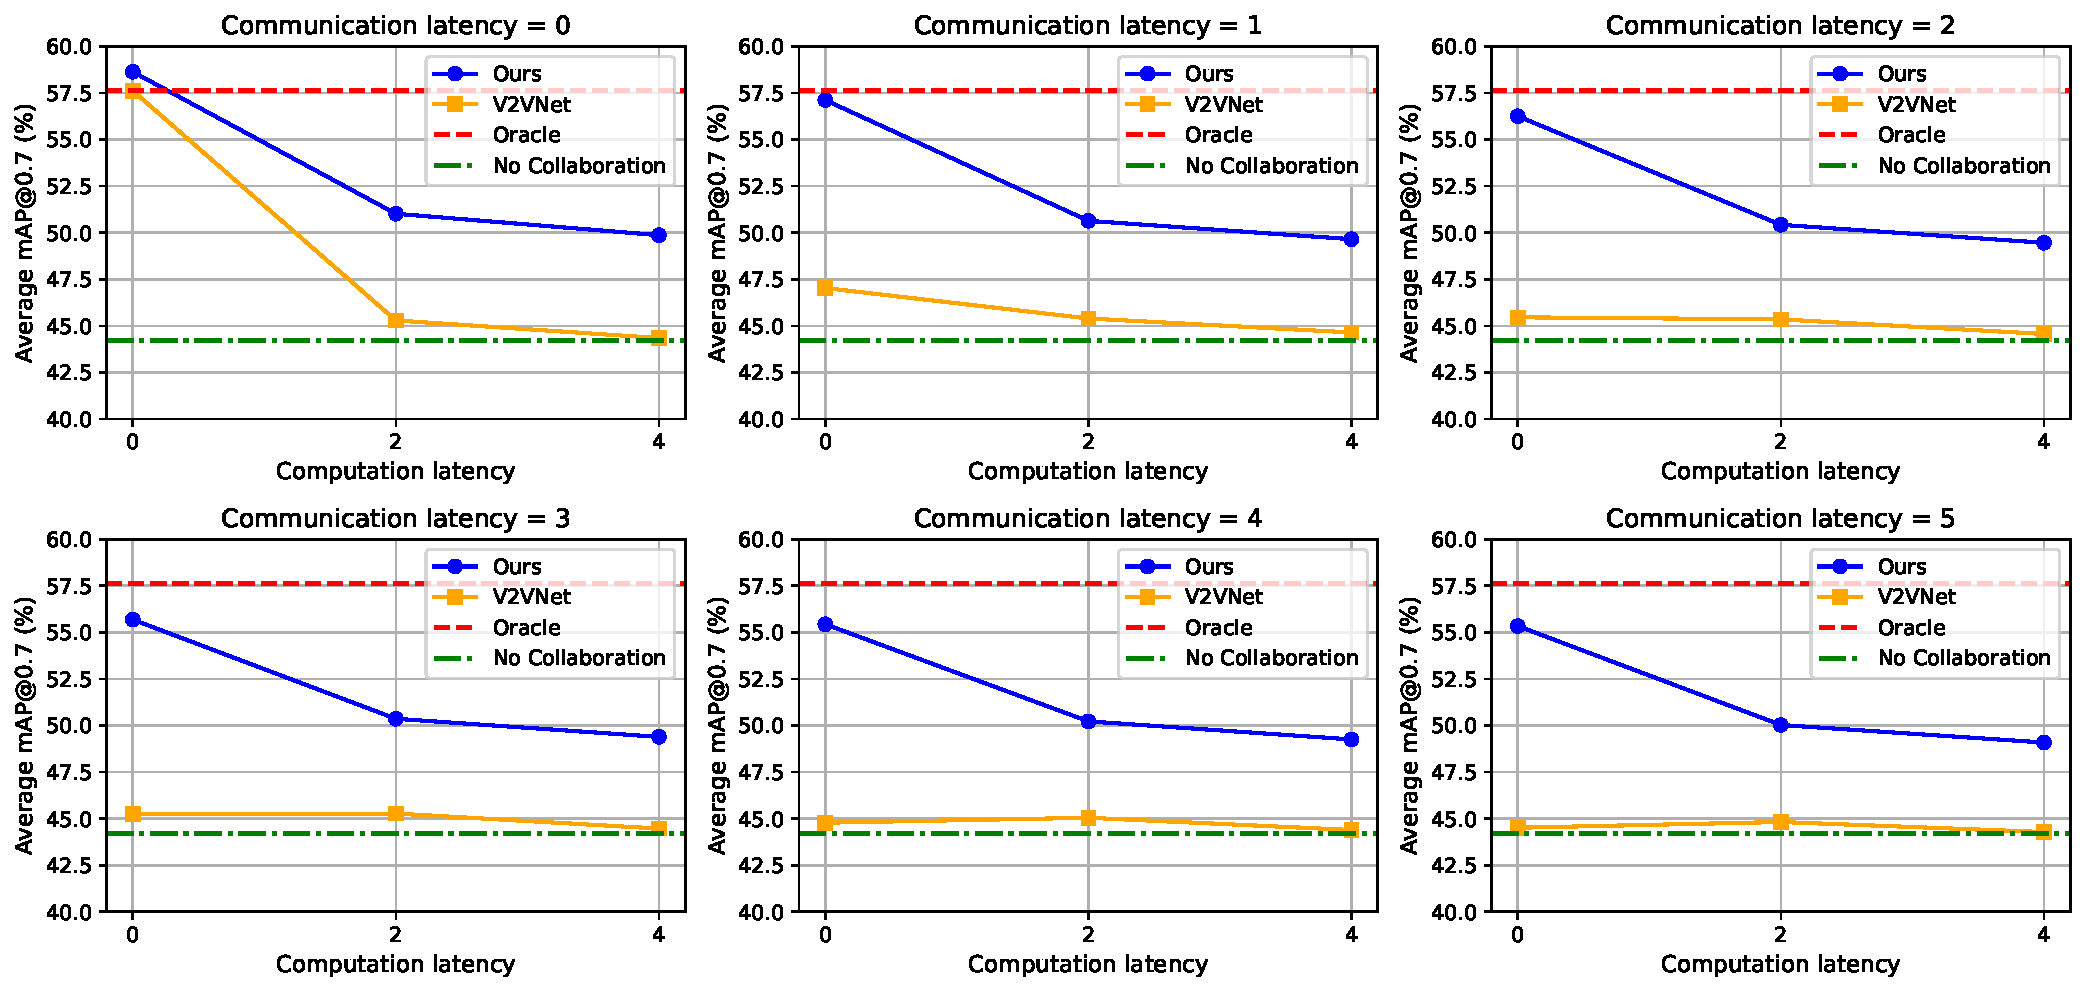
\includegraphics[width=0.95\linewidth]{pics/main_compare.pdf}
    \caption{Comparison of mAP@0.7 under varying communication and computation latency settings on the V2X-Sim dataset. Our method consistently outperforms the V2VNet baseline across all latency conditions and even surpasses the Oracle in the zero-latency scenario by leveraging richer historical information. Latency is measured in frames, with each frame representing 0.2 seconds.
    }
    \label{fig:0.7_lat}
\end{figure*}

\begin{figure*}[t]
    \centering
    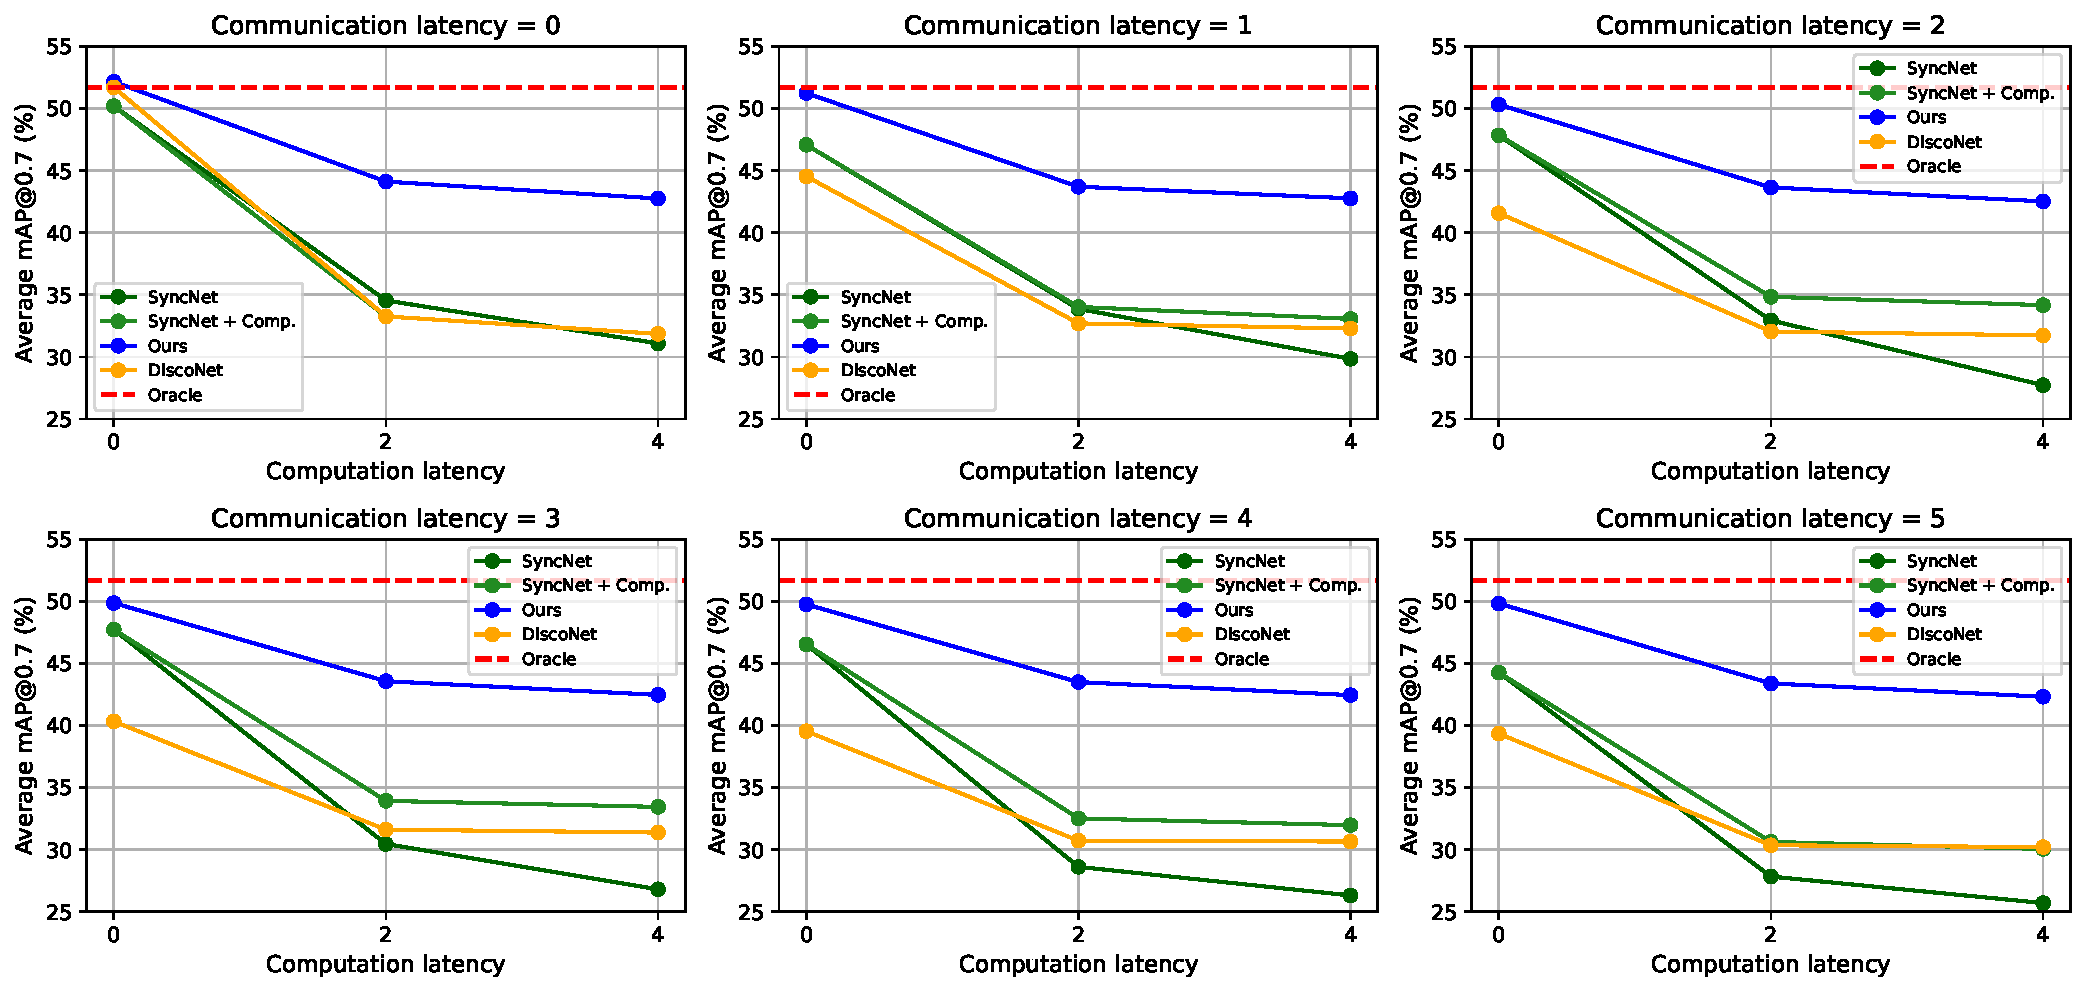
\includegraphics[width=0.95\linewidth]{pics/compare_disco-07}
    \caption{Comparison of mAP@0.7 under varying communication and computation latency settings on the V2X-Sim dataset. We compare four approaches: SyncNet, SyncNet + Comp., DiscoNet, Ours, and Oracle. Since the original SyncNet does not account for computation latency, we additionally present its extended results where computation latency is considered to provide a more comprehensive comparison. Latency is measured in frames, with each frame representing 0.2 seconds.
    }
    \label{fig:compare_syn}
\end{figure*}


\subsubsection{\textbf{Model State Transmission}}\\

We then investigate the efficiency gains brought by transmitting only compressed model states instead of feature-level data. Two aspects are considered: (i) the reduction of communication bandwidth consumption, and (ii) the alleviation of redundant computation at the receiver side. Both aspects are reported in tabular form to provide a clear quantitative comparison.
\paragraph{Changes in Communication Pressure}
\begin{table}[ht]
\centering
\caption{Comparison of Communication Pressure: Feature-Level Data vs. Compressed Model States}
\begin{tabular}{lcc}
\toprule
\textbf{Communication Data Type} & \textbf{Transmission Size} & \textbf{Reduction} \\
\midrule
Feature-Level Data & 1.9MB & - \\
Compressed Model States & 0.65MB & 65\% \\
\bottomrule
\end{tabular}

\label{tab:communication_pressure_comparison}
\end{table}

By compressing the model states and transmitting them instead of the feature-level data, we significantly alleviate the communication pressure. Specifically, in the Table~\ref{tab:communication_pressure_comparison}, the feature-level data (1.9MB) represents the data after fusing and processing perception information from multiple sensors of a transmitting vehicle. Using the int8pc compression method with temporal differencing, we reduced the size of the transmitted model states to 0.65MB (with an Normalized Mean Squared Error(NMSE) of 0.0054\%), resulting in a reduction of approximately 65\% in communication volume. This V2X-Sim comparison reports the original feature-level transmission setting, while the later DAIR-V2X-C MST table reports recurrent-state variants under a separate state-size profiling protocol. The two numbers therefore quantify different transmission formats rather than conflicting measurements. This transmission mechanism not only effectively reduces communication pressure but also provides the system with richer information, leading to more precise predictive compensation. 


\paragraph{Reducing Redundant Computation}
In this work, we propose a strategy where the encoder computation is offloaded to the transmitting vehicle, while the decoder computation is handled by the receiving vehicles. This distribution of computation has several key advantages in terms of reducing redundant computational load, particularly in a multi-agent system. 
When both the encoder and decoder computations are performed by each receiving vehicle, the redundancy increases with the number of receiving vehicles. Specifically, for each additional receiving vehicle, the encoder computation must be repeated, thereby leading to significant computational overhead. This redundancy becomes more pronounced as the number of receiving vehicles increases. In contrast, by offloading the encoder to the transmitting vehicle, only a single vehicle performs the encoder operation, while the receiving vehicles only execute the decoder. This leads to a significant reduction in computational redundancy.
In our method, the encoder computation is roughly 3 times more computationally expensive than the decoder computation (Table~\ref{tab:redundant_computation_comparison}). So, if we have a system with 5 vehicles, and 4 of them are receiving vehicles, the redundancy caused by the repeated execution of the encoder operation across these receiving vehicles results in a total computational overhead equivalent to three times the encoder's calculation. This redundancy represents about 57.1\% of the total computational load in the system. Therefore, by offloading the encoder to the transmitting vehicle and allowing only the decoder to run on the receiving vehicles, we achieve a significant reduction in computational redundancy, optimizing overall system efficiency.

%encoder：1600000flops decoder：50000flops Redundant encoder computation=3×1,600,000=4,800,000FLOPs  Total computation for 4 receiving vehicles=4×2,100,000=8,400,000FLOPs  48/84=57.1%
\begin{table}[ht]
\centering
\caption{Comparison of Redundant Computation in the System}
\begin{tabular}{lcc}
\toprule
\textbf{Computation Type} & \textbf{Computation (MFLOPs)} \\
\midrule
Encoder (per vehicle) & 1.6 \\
Decoder (per vehicle) & 0.5 \\
Redundant Encoder (for 3 vehicles) & 4.8 \\
Total (for 4 receiving vehicles) & 8.4 \\
\midrule
Redundant Percentage & 57.1\% \\
\bottomrule
\end{tabular}
\label{tab:redundant_computation_comparison}
\end{table}

%FLOPs stands for Floating Point Operations, which is a measure of computational performance. It refers to the number of mathematical operations (such as additions, multiplications, etc.) involving floating-point numbers that are performed by a processor or algorithm.

\subsubsection{\textbf{Dual-latency Perceptive Compensation Fusion}}
Finally, we evaluate the end-to-end performance of cooperative perception under dual-latency settings, i.e., simultaneous communication and computation latencies. To better approximate real-world deployment, we vary the latency configurations to emulate different compression ratios. Our method is compared against four baselines: SyncNet~\cite{lei2022latency}, an oracle (ideal V2VNet~\cite{wang2020v2vnet} or DiscoNet~\cite{li2021learning} without latency), a lower-bound (V2VNet~\cite{wang2020v2vnet} or DiscoNet~\cite{li2021learning} with latency but without compensation), and the single-agent V2VNet~\cite{wang2020v2vnet} or DiscoNet~\cite{li2021learning} without cooperation. Results are reported in terms of AP@0.5/0.7 across all latency settings. Both tabular and graphical comparisons demonstrate that the proposed transmitter-side compensation achieves consistently superior performance in diverse latency scenarios.

\begin{table*}[t]
\centering
\caption{Comparison of mAP@0.5 and mAP@0.7 under different \emph{communication and computation latency} settings on the V2X\textendash Sim dataset. Oracle is reported only at the AVG columns (others are unavailable, shown as ``--'').}
\begin{tabular}{c c *{14}{c}}
\toprule
\multirow{2}{*}{\textbf{Method}} & &
\multicolumn{7}{c}{\textbf{AP@0.5}} &
\multicolumn{7}{c}{\textbf{AP@0.7}} \\
\cmidrule(lr){3-9}\cmidrule(lr){10-16}
& \multicolumn{1}{c}{\diagbox{\small{Comp.}}{\small{Comm.}}} &
\textbf{AVG} & \textbf{0} & \textbf{1} & \textbf{2} & \textbf{3} & \textbf{4} & \textbf{5} &
\textbf{AVG} & \textbf{0} & \textbf{1} & \textbf{2} & \textbf{3} & \textbf{4} & \textbf{5} \\
\midrule
\textbf{Oracle} & -- &
\textit{56.62} & -- & -- & -- & -- & -- & -- &
\textit{51.70} & -- & -- & -- & -- & -- & -- \\
\midrule
\multirow{3}{*}{\textbf{SyncNet}} & 0 &
55.07 & 56.62 & 53.49 & 55.73 & 55.72 & 54.90 & 52.56 &
47.27 & 50.20 & 47.08 & 47.84 & 47.72 & 46.53 & 44.26 \\
& 2 &
38.34 & 41.14 & 40.98 & 40.04 & 37.87 & 35.60 & 34.41 &
31.38 & 34.55 & 33.87 & 32.94 & 30.45 & 28.62 & 27.83 \\
& 4 &
34.62 & 37.91 & 36.46 & 34.72 & 33.89 & 32.83 & 31.90 &
27.91 & 31.09 & 29.84 & 27.73 & 26.81 & 26.31 & 25.70 \\
\midrule
\multirow{3}{*}{\textbf{SyncNet w/ Comp.}} & 0 &
55.07 & 56.62 & 53.49 & 55.73 & 55.72 & 54.90 & 52.56 &
47.27 & 50.20 & 47.08 & 47.84 & 47.72 & 46.53 & 44.26 \\
& 2 &
39.94 & 41.25 & 39.73 & 41.52 & 40.53 & 39.28 & 37.35 &
33.20 & 33.26 & 34.02 & 34.84 & 33.93 & 32.52 & 30.62 \\
& 4 &
38.55 & 38.65 & 38.25 & 40.34 & 39.53 & 38.21 & 36.31 &
32.43 & 31.86 & 33.06 & 34.17 & 33.44 & 31.97 & 30.06 \\
\midrule
\multirow{3}{*}{\textbf{DiscoNet}} & 0 &
51.46 & 56.62 & 54.88 & 51.24 & 49.46 & 48.60 & 47.94 &
42.84 & 51.70 & 44.53 & 41.57 & 40.32 & 39.54 & 39.34 \\
& 2 &
39.19 & 41.25 & 41.03 & 39.75 & 38.91 & 37.38 & 36.80 &
31.78 & 33.26 & 32.70 & 32.05 & 31.61 & 30.72 & 30.36 \\
& 4 &
37.87 & 38.65 & 39.41 & 38.35 & 37.70 & 36.85 & 36.25 &
31.35 & 31.86 & 32.29 & 31.73 & 31.38 & 30.65 & 30.21 \\
\midrule
\multirow{3}{*}{\textbf{Ours}} & 0 &
54.52 & 56.83 & 55.09 & 54.11 & 53.83 & 53.56 & 53.70 &
50.52 & 52.16 & 51.24 & 50.32 & 49.86 & 49.75 & 49.82 \\
& 2 &
48.15 & 48.59 & 48.22 & 48.16 & 48.11 & 47.92 & 47.89 &
43.65 & 44.11 & 43.70 & 43.65 & 43.57 & 43.49 & 43.39 \\
& 4 &
46.99 & 47.31 & 47.13 & 46.95 & 46.98 & 46.85 & 46.75 &
42.54 & 42.75 & 42.77 & 42.52 & 42.46 & 42.44 & 42.31 \\
\bottomrule
\end{tabular}
\label{tab:map-upper-lower-disco}
\end{table*}

%In Table~\ref{tab:map-upper-lower}, we present a comprehensive performance comparison between our method based on V2VNet~\cite{wang2020v2vnet} and various baselines under different \emph{communication} and \emph{computation} latency settings. The reported mAP@0.5 and mAP@0.7 are averaged over all test cases, considering Communication latency = 0--5 and Computation latency = 0--4. Overall, our method consistently achieves superior performance across all latency conditions. Specifically, compared to the V2VNet baseline, our approach improves the averaged mAP@0.5 by approximately \textbf{3\%--7\%} and the averaged mAP@0.7 by approximately \textbf{5\%--10\%}, demonstrating its robustness under various latency scenarios.

In Table~\ref{tab:map-upper-lower-v2v}, we present a comprehensive performance comparison between our method based on V2VNet~\cite{wang2020v2vnet} and various baselines under different \emph{communication} and \emph{computation} latency settings. The reported mAP@0.5 and mAP@0.7 are averaged over all test cases, considering Communication latency = 0--5 and Computation latency = 0--4.

From the V2VNet~\cite{wang2020v2vnet} results, it can be seen that as the computation latency increases, the performance of V2VNet without the dual-latency prediction compensation mechanism declines significantly. Even with just a 2-frame computation latency, there is a considerable performance fluctuation, with a nearly \textbf{12\%} drop in AP@0.7. Under computation latency = 4 and communication latency = 5, the AP@0.7 results of V2VNet without compensation are already very close to the results of no collaboration. These findings highlight that in cooperative perception scenarios, both communication latency and computation latency are crucial issues that cannot be overlooked, effectively demonstrating the significance of our dual-latency prediction compensation mechanism.

Meanwhile, our method consistently achieves superior performance across all latency conditions. Specifically, compared to the V2VNet baseline, our approach improves the averaged mAP@0.5 by approximately \textbf{3\%--7\%} and the averaged mAP@0.7 by approximately \textbf{5\%--9\%}, demonstrating its robustness under various latency scenarios. Even in adverse conditions with a communication latency of 5, our dual-latency compensation mechanism improves the V2VNet baseline by about \textbf{10\%}, falling short of the ideal scenario by \textbf{less than 2\%}. Additionally, when the computation latency is significantly large at 4, our framework achieves a 5.52\% improvement in AP@0.7, effectively proving that our dual-latency prediction compensation mechanism greatly enhances the robustness of V2VNet under dual latency conditions.


Furthermore, as illustrated in Figure~\ref{fig:0.7_lat}, which vividly showcases the data from Table~\ref{tab:map-upper-lower-v2v}, our method even \emph{surpasses the Oracle performance} in the ideal zero-latency scenario. This notable gain can be attributed to leveraging \emph{richer historical information}, which provides additional context for collaborative perception and mitigates temporal inconsistency. Importantly, under \emph{all} latency settings, our method maintains a consistent performance advantage over the V2VNet baseline, confirming its effectiveness in handling delayed information. Moreover, we can observe that when the communication latency is greater than 1 and the computation latency is present, the results of the V2VNet baseline are very close to those of no collaboration, which diminishes the benefits of inter-agent communication. The results once again emphasize the significant impact of dual latency on the accuracy of cooperative perception.

%It is also worth noting that when computation latency is ignored, the performance of V2VNet approaches the lower bound established by the No Collaboration setting. This observation highlights the \emph{critical importance of accounting for computation latency} when designing collaborative perception systems, as neglecting it can significantly diminish the benefits of inter-agent communication.
%In Figure~\ref{fig:compare_syn}, we compare our compensation mechanism with SyncNet~\cite{lei2022latency} on DiscoNet~\cite{li2021learning} under different communication and computation latency settings. The original SyncNet does not account for computation latency in its design. To provide a fair and comprehensive comparison, we evaluate two variants of SyncNet: one that strictly follows the original implementation and another extended version, SyncNet+Comp, where computation latency is explicitly considered. The results demonstrate that our method consistently outperforms both SyncNet variants under nearly all latency conditions. Moreover, SyncNet+Comp achieves superior performance compared to the original SyncNet in the vast majority of scenarios, underscoring the significance of properly modeling computation latency for collaborative perception.
In Table~\ref{tab:map-upper-lower-disco}, we further present the results based on DiscoNet~\cite{li2021learning} and compare them against multiple baselines. Consistent with the findings on V2VNet~\cite{wang2020v2vnet}, the performance of the original DiscoNet degrades significantly as the computation and communication latencies increase, highlighting that the impact of both communication and computation latency on system performance is not an isolated phenomenon in cooperative perception.

In contrast, our method consistently demonstrates stable advantages across all latency configurations. On average, our approach improves the baseline DiscoNet by approximately \textbf{3\%--9\%} in mAP@0.5 and \textbf{8\%--12\%} in mAP@0.7, further validating the effectiveness of the proposed dual-latency prediction compensation mechanism in enhancing robustness. Even under the extreme condition of communication latency = 5 and computation latency = 4, our method maintains a clear margin over the baseline, underscoring its resilience in challenging latency environments.

To further evaluate the effectiveness of our framework, we also compare it with SyncNet~\cite{lei2022latency} and its extended variant SyncNet+Comp. As shown in Table~\ref{tab:map-upper-lower-disco}, the original SyncNet does not account for computation latency in its design, and thus its performance drops rapidly as latency grows. In contrast, SyncNet+Comp achieves noticeable improvements over the original SyncNet in most scenarios, verifying the importance of explicitly modeling computation latency. Nevertheless, our method consistently outperforms both SyncNet variants under all latency conditions, further demonstrating the generality and superiority of the proposed compensation mechanism.

In Figure~\ref{fig:compare_syn}, we illustrate the trends of mAP@0.7 under different communication latencies as computation latency increases. The results clearly indicate that the performance of SyncNet degrades sharply under high-latency conditions, whereas our framework consistently sustains a higher level of accuracy. This observation not only confirms the adaptability of the proposed dual-latency prediction compensation mechanism to DiscoNet but also reinforces the critical importance of dual-latency modeling for collaborative perception.

In summary, whether built upon V2VNet~\cite{wang2020v2vnet} or DiscoNet~\cite{li2021learning}, our method consistently demonstrates significant and robust advantages under dual-latency settings. Compared to existing approaches, the proposed compensation mechanism effectively mitigates performance degradation across diverse latency configurations while maintaining high perception accuracy. More importantly, even under complex and adverse latency conditions, our framework continues to deliver stable improvements over baseline methods, fully validating its practicality and robustness for real-world deployment.

\subsubsection{\textbf{DAIR-V2X-C Real-World Validation}}
To further examine whether the proposed mechanism remains valid beyond the simulated V2X-Sim setting, we conduct additional experiments on DAIR-V2X-C. This part contains two complementary evaluations. First, we run official cooperative detection baselines to quantify how real DAIR point-cloud detection performance changes with communication delay. Second, we evaluate our VSPM and MST components on DAIR annotation-derived BEV occupancy sequences, which allows the same latency-compensation logic and prediction metrics to be tested on real cooperative scenes. These two DAIR evaluations use different metrics and should be interpreted separately: the official baselines report detection AP, while our DAIR VSPM/MST evaluation reports BEV forecasting IoU and does not claim end-to-end detection AP for our method.

\begin{table*}[t]
\centering
\scriptsize
\caption{Representative DAIR-V2X-C official detection baselines. Delay is measured in frames.}
\label{tab:dair-official-baselines}
\begin{tabular}{lrrrrrr}
\toprule
Method & $k$ & 3D@0.5 & 3D@0.7 & BEV@0.5 & BEV@0.7 & Comm. B \\
\midrule
Vehicle only & 0 & 48.03 & 35.08 & 52.24 & 46.51 & 0.00 \\
Infrastructure only & 0 & 17.60 & 7.06 & 27.34 & 14.42 & 478.56 \\
Late fusion + TCLF & 0 & 55.98 & 40.01 & 62.00 & 54.11 & 911.96 \\
Late fusion + TCLF & 3 & 52.14 & 36.57 & 57.80 & 49.46 & 885.55 \\
Late fusion + TCLF & 5 & 51.29 & 36.30 & 56.75 & 48.71 & 861.65 \\
Late fusion w/o comp. & 1 & 53.73 & 36.88 & 59.90 & 50.11 & 478.76 \\
Late fusion w/o comp. & 3 & 51.36 & 36.25 & 56.90 & 48.80 & 477.40 \\
Late fusion w/o comp. & 5 & 50.87 & 36.17 & 56.18 & 48.36 & 466.53 \\
Early fusion & 0 & 62.61 & 37.50 & 68.94 & 59.02 & 2284.16 \\
Early fusion & 2 & 54.62 & 32.17 & 61.07 & 50.04 & 2316.11 \\
Early fusion & 5 & 50.93 & 30.98 & 56.47 & 46.99 & 2496.60 \\
\bottomrule
\end{tabular}
\end{table*}


\begin{figure}[t]
    \centering
    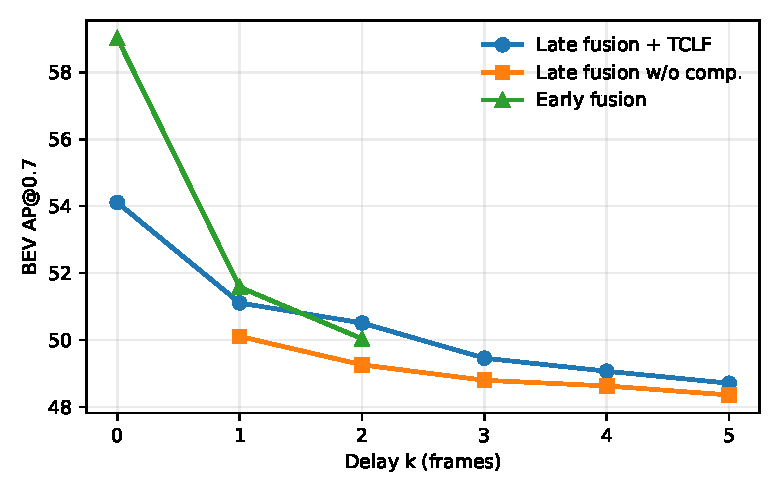
\includegraphics[width=0.95\linewidth]{pics/dair_official_delay.pdf}
    \caption{BEV AP@0.7 of DAIR-V2X-C official detection baselines under different delay settings. The results show that real cooperative detection accuracy degrades as stale information is used, while time-compensated late fusion remains more stable than uncompensated late fusion at larger delays.}
    \label{fig:dair-official-delay}
\end{figure}

Table~\ref{tab:dair-official-baselines} and Fig.~\ref{fig:dair-official-delay} summarize representative DAIR-V2X-C official detection results. Compared with vehicle-only perception, cooperative fusion improves both 3D and BEV AP, confirming the value of V2X information in real scenes. At the same time, the degradation from $k=0$ to larger delay values shows that delayed cooperative messages do hurt detection accuracy. The time-compensated late-fusion (TCLF) baseline maintains higher BEV AP@0.7 than the uncompensated late-fusion baseline at larger delays, which supports the central motivation of explicitly modeling latency in real cooperative perception. Early fusion is used here as a high-communication official reference rather than as a strict upper bound, since its performance also degrades under large delay.

\begin{table*}[t]
\centering
\scriptsize
\caption{DAIR-V2X label-derived BEV delay and system ablation.}
\label{tab:dair-delay-system}
\begin{tabular}{llrrrrr}
\toprule
Setting & Mode & Cases & IoU & Copy & $\Delta$IoU & Dyn. IoU \\
\midrule
T10\_n10 ckpt 15000 & no\_comp & 30 & 0.1945 & 0.1945 & 0.0000 & 0.0497 \\
T10\_n10 ckpt 15000 & comm\_only & 30 & 0.2960 & 0.1945 & 0.1015 & 0.2380 \\
T10\_n10 ckpt 15000 & comp\_only & 30 & 0.2784 & 0.1945 & 0.0839 & 0.2053 \\
T10\_n10 ckpt 15000 & dual & 30 & 0.4097 & 0.1945 & 0.2153 & 0.4436 \\
T10\_n10 ckpt 15000 & oracle & 30 & 1.0000 & 0.1945 & 0.8055 & 1.0000 \\
T10\_n5 ckpt 16000 & no\_comp & 15 & 0.2857 & 0.2857 & 0.0000 & 0.0836 \\
T10\_n5 ckpt 16000 & comm\_only & 15 & 0.3956 & 0.2857 & 0.1099 & 0.2672 \\
T10\_n5 ckpt 16000 & comp\_only & 15 & 0.3956 & 0.2857 & 0.1099 & 0.2672 \\
T10\_n5 ckpt 16000 & dual & 15 & 0.5207 & 0.2857 & 0.2350 & 0.4830 \\
T10\_n5 ckpt 16000 & oracle & 15 & 1.0000 & 0.2857 & 0.7143 & 1.0000 \\
\bottomrule
\end{tabular}
\end{table*}


\begin{figure}[t]
    \centering
    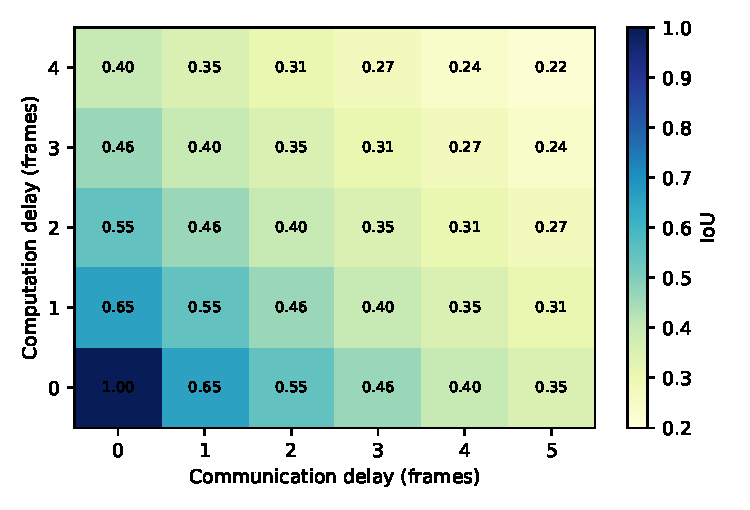
\includegraphics[width=0.95\linewidth]{pics/dair_delay_heatmap.pdf}
    \caption{DAIR-V2X-C label-derived BEV IoU of the proposed dual-latency compensation under the full $T10\_n10$ latency grid. The x-axis is communication delay and the y-axis is computation delay, both measured in frames.}
    \label{fig:dair-delay-heatmap}
\end{figure}

Table~\ref{tab:dair-delay-system} reports the system-level DAIR delay ablation. For the full $T10\_n10$ setting, the dual-latency mode achieves an average IoU of 0.4097, compared with 0.1945 for no compensation, 0.2960 for communication-only compensation, and 0.2784 for computation-only compensation. This full-grid setting is the main evidence for separating communication-only, computation-only, and joint compensation. For the shorter $T10\_n5$ setting, the supported latency subset is symmetric for the single-delay modes, so we use it primarily as a short-horizon confirmation: the dual-latency mode reaches 0.5207 IoU and improves over the no-compensation setting by 0.2350 IoU. These results demonstrate that communication and computation delays should be compensated jointly rather than treated as isolated effects. Fig.~\ref{fig:dair-delay-heatmap} further shows the expected trend that prediction difficulty increases as the total target horizon becomes larger.

\begin{table}[t]
\centering
\scriptsize
\caption{MST communication-state trade-off on DAIR-V2X label-derived BEV.}
\label{tab:dair-mst-tradeoff}
\begin{tabular}{lrrrrrr}
\toprule
Variant & MiB/agent & Reduction & ms & IoU & $\Delta$IoU & Dyn. IoU \\
\midrule
ConvLSTM state & 16.000 & 1.0$\times$ & 3.59 & 0.5188 & 0.2469 & 0.4646 \\
GRU FP16 & 4.000 & 4.0$\times$ & 4.40 & 0.5551 & 0.2833 & 0.5240 \\
DS64 FP16 & 0.250 & 64.0$\times$ & 4.21 & 0.6066 & 0.3348 & 0.5888 \\
Bottleneck12 & 0.250 & 64.0$\times$ & 4.31 & 0.6021 & 0.3302 & 0.5682 \\
\bottomrule
\end{tabular}
\end{table}


\begin{figure}[t]
    \centering
    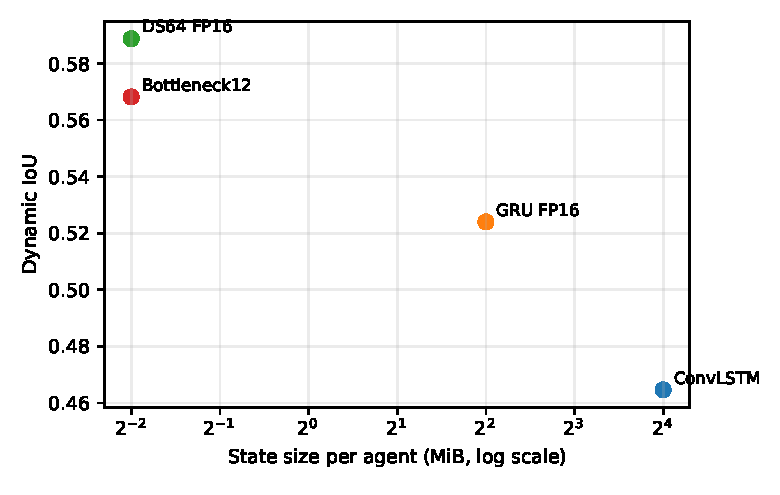
\includegraphics[width=0.95\linewidth]{pics/dair_mst_pareto.pdf}
    \caption{Bandwidth-performance trade-off of MST variants on DAIR-V2X-C label-derived BEV. Smaller state size reduces communication and cache pressure; Dynamic IoU reports prediction quality on changed BEV regions.}
    \label{fig:dair-mst-pareto}
\end{figure}

Table~\ref{tab:dair-mst-tradeoff} and Fig.~\ref{fig:dair-mst-pareto} analyze whether MST reduces communication-state cost without invalidating prediction quality. The original ConvLSTM hidden and cell states require 16.0 MiB per agent. The DS64-FP16 and Bottleneck12 variants reduce the recurrent state to 0.25 MiB per agent, corresponding to a $64\times$ reduction, while achieving higher IoU and Dynamic IoU than the uncompressed ConvLSTM-state baseline. This 0.25 MiB/agent value is the profiled DAIR recurrent-state footprint, whereas Table~\ref{tab:communication_pressure_comparison} reports a separate V2X-Sim feature-level transmission comparison. This indicates that the transmitted state can be compact while still preserving the temporal information needed for compensation.

\begin{table}[t]
\centering
\scriptsize
\caption{History length and rollout-horizon sensitivity on DAIR-V2X label-derived BEV.}
\label{tab:dair-sensitivity}
\begin{tabular}{lrrrr}
\toprule
Setting & Best step & IoU & $\Delta$IoU & Dyn. IoU \\
\midrule
T5\_n5 & 16650 & 0.5183 & 0.2464 & 0.4427 \\
our\_method\_T10\_n5 & 16140 & 0.5164 & 0.2446 & 0.4465 \\
T20\_n5 & 28000 & 0.5237 & 0.2522 & 0.4564 \\
T30\_n5 & 52000 & 0.5230 & 0.2519 & 0.4741 \\
T10\_n3 & 16350 & 0.5954 & 0.2229 & 0.4318 \\
our\_method\_T10\_n10 & 15630 & 0.3853 & 0.2105 & 0.3834 \\
T10\_n15 & 29000 & 0.3065 & 0.1722 & 0.3385 \\
\bottomrule
\end{tabular}
\end{table}


Table~\ref{tab:dair-sensitivity} studies the sensitivity to history length $T$ and prediction rollout horizon $n$. With $n=5$, increasing $T$ from 5 to 20 or 30 provides only moderate changes, which suggests that the default history length is not a fragile choice. In contrast, increasing the rollout horizon from $n=3$ to $n=10$ or $n=15$ clearly lowers absolute IoU, because long-horizon BEV forecasting is harder and covers larger communication/computation delay. This trend is consistent with the latency heatmap and explains why the short-horizon model is used for high-accuracy compensation while the $T10\_n10$ model is used to cover the full delay grid.

\begin{table*}[t]
\centering
\scriptsize
\caption{Robustness of DAIR-V2X VSPM under packet loss and BEV perturbations.}
\label{tab:dair-robustness}
\begin{tabular}{llrrrr}
\toprule
Setting & Condition & IoU & Copy & $\Delta$IoU & Dyn. IoU \\
\midrule
T10\_n5 ckpt 16000 & clean & 0.5478 & 0.2771 & 0.2707 & 0.4733 \\
T10\_n5 ckpt 16000 & packet\_loss\_0.3 & 0.4411 & 0.2443 & 0.1968 & 0.3490 \\
T10\_n5 ckpt 16000 & packet\_loss\_0.5 & 0.3476 & 0.2126 & 0.1351 & 0.2497 \\
T10\_n5 ckpt 16000 & dropout\_0.2 & 0.4867 & 0.2368 & 0.2500 & 0.4436 \\
T10\_n5 ckpt 16000 & false\_positive\_0.005 & 0.5082 & 0.2140 & 0.2942 & 0.4268 \\
T10\_n10 ckpt 15000 & clean & 0.4057 & 0.1709 & 0.2348 & 0.4291 \\
T10\_n10 ckpt 15000 & packet\_loss\_0.3 & 0.3261 & 0.1540 & 0.1721 & 0.3267 \\
T10\_n10 ckpt 15000 & packet\_loss\_0.5 & 0.2569 & 0.1366 & 0.1203 & 0.2413 \\
T10\_n10 ckpt 15000 & dropout\_0.2 & 0.3742 & 0.1471 & 0.2271 & 0.4050 \\
T10\_n10 ckpt 15000 & false\_positive\_0.005 & 0.3833 & 0.1357 & 0.2476 & 0.3755 \\
\bottomrule
\end{tabular}
\end{table*}


\begin{figure}[t]
    \centering
    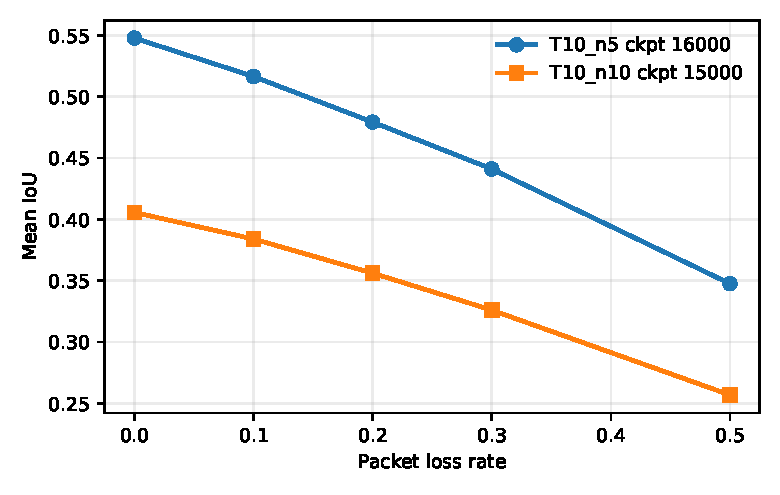
\includegraphics[width=0.95\linewidth]{pics/dair_packet_loss.pdf}
    \caption{DAIR-V2X-C VSPM robustness under packet loss. Performance degrades smoothly as packet loss increases, while the prediction model keeps positive gains over the copy-last-frame baseline in Table~\ref{tab:dair-robustness}.}
    \label{fig:dair-packet-loss}
\end{figure}

Finally, Table~\ref{tab:dair-robustness} and Fig.~\ref{fig:dair-packet-loss} evaluate robustness under packet loss, BEV dropout, and false positives. The mean IoU decreases as packet loss increases, which is expected because less historical information is available for stable prediction. Nevertheless, the IoU gain over the copy-last-frame baseline remains positive under all tested perturbations. This result indicates that DLPCM is not invariant to sensing and communication noise, but its degradation is gradual and remains explainable under realistic disturbances.
